\documentclass[12pt, a4paper]{report} \usepackage[titletoc]{appendix}
\usepackage{graphicx}
	\graphicspath{{images/}} 
\usepackage{geometry}
	\geometry{a4paper,left=3cm,top=3cm,bottom=3cm,right=3cm}
\usepackage{array}
\usepackage{multirow}
\usepackage{hyperref}
	\hypersetup{colorlinks=true,allcolors=blue}
\usepackage{hypcap}
\usepackage{csquotes}
\usepackage{subfig}

\setlength{\parindent}{1cm}
\setlength{\parskip}{0.1cm}


\begin{document}

\begin{titlepage}
 \begin{center}

\textbf{Progress Report}
\vspace{1cm}

\textbf{\large Model-Driven Gamified Software Modelling Learning}
\vspace{1cm}

Alfa Ryano Yohannis\\
ary506@york.ac.uk
\vspace{1cm}

Supervisors:\\
Dimitris Kolovos\\
Fiona Polack\\
\vspace{1cm}

Department of Computer Science\\
University of York\\
United Kingdom\\
\vspace{1cm}
\today
 
\vfill
 
\end{center}
\end{titlepage}


\begin{abstract}
\addcontentsline{toc}{chapter}{Abstract}
In software engineering, software modelling plays a significant role.
Nevertheless, learners often consider software modelling as a comparatively 
difficult subject since it requires them to have abstraction skills to master it. Meanwhile, gamification has been growing as a trend solution to improving learners' engagement. This study endeavours to harness Model-Driven Engineering best practices to construct gamified learning activities that supports learners advancing their modelling abilities. Our method to dealing with the gamified learning combines pedagogical design principles derived from several learning models and the Deterding's Gameful Design framework for it's gamification. Using the Design Science Research Methodology, this research aims to produce a framework for designing and generating gamified software modelling learning. Controlled experiments are planned to be applied to evaluate the effectiveness of the framework as well as the gamified software modelling learning produced.
\end{abstract}

\tableofcontents
\addcontentsline{toc}{chapter}{Contents}

\chapter{Introduction}
\label{Introduction}
In this section, the background, questions, objectives, potential outputs, and scoping of this research are presented.

\section{Background}
Software modelling is commonly perceived as a difficult subject since it
requires a mastery of abstraction \cite{Borstler2012}. However, this subject
has a significant role in software engineering education and
practice. Successful application of software modelling requires skills in
abstract modelling \cite{whittle2013industrial}. The modelling itself is the
process of thinking abstractly about systems \cite{bezivin2009teaching}. Thus,
teaching modelling also means teaching abstraction \cite{engels2005teaching}.
Therefore, it is crucial to make students understand the value of abstraction
\cite{bezivin2009teaching}. Weak software modelling skills will likely cause
software engineering students to face further challenges with their degrees, as
most of the software engineering related subjects involve of inherent
abstraction problems \cite{Kramer2007}. Drawing from multidiciplinary research to define abstraction for Artifical Intelligence, Saitta et al. stated that abstraction is often associated with these processes: information hiding, generalisation, approximation or reformulation, and separating relevant from irrelevant aspects \cite{Saitta2013}. Those processes are the common approaches applied in Computer Science, such as encapsulation and generalization in object-oriented programming, resolution of polygon density in 3D modelling, algebraic simplication in symbolic computation, and removing colour information of images to produce grayscales. In the context of software engineering and computer science education, Kramer \cite{Kramer2007} and Hazzan \cite{hazzan2008reflections} argued that abstraction is the central theme or key
skill for computing.

\begin{displayquote}
``I believe that abstraction is a key skill for computing. It is essential
during requirements engineering to elicit the critical aspects of the 
environment \dots At design time \dots Even at the implementation stage
\dots --- Kramer \cite{Kramer2007}.
\end{displayquote}

\begin{displayquote}
`` \dots software is an intangible object, and hence, requires highly developed
cognitive skills for coping with different levels of abstraction." --- Hazzan
\cite{hazzan2008reflections}.
\end{displayquote}

The problem of learning appropriate abstraction skills for software modelling is similar to problems in mathematics, where most of the concepts can only be accessed through symbolical representations \cite{Duval2006}. The abstract nature of software modelling traditionally has been addressed through the use of diagrams or visual notations in the form of modelling and diagramming tools. However, grasping concepts represented by the visual notations and conversely presenting back the concepts into visual notations are not trivial, including presenting aspects of the concept in different visual notation as well as choosing the right levels of abstraction and moving between them. Learning and teaching these skills is challenging and to overcome the challenges, a dedicated framework to support the learning of the modelling skills in a gamified way will bring great benefits. 
 
The presence of learning framework does not guarantee will improve learners' engagement in software modelling learning. In recent years, the use of games and game elements, such as Gamification \cite{deterding2011game} and Serious Games \cite{Michael2005}, for purposes other than leisure has drawn significant attention. Gamified approaches have been proposed as solutions to motivational problems that emerge when users are required to engage in activities that they perceive as boring, irrelevant, or difficult. 

Real-world examples that show the success of the gamification are Duolingo\footnote{\url{https://www.duolingo.com/ }} and Re-mission\footnote{\url{http://www.re-mission.net/}}. Duolingo is a gamified system of language learning. It embeds game elements, such as points, levels,and lives, to make language learning more fun. Re-mission is a third-person shooting game dedicated to young cancer patients and designed to teach and learn how to deal with cancer. The patients are invited to take part in an entertaining gameplay that will affect their specific behavioural and psychological outcomes producing effective cancer therapy.
 
Through a systematic review, Connolly et al. \cite{connolly2012systematic} studied the impact of computer games and serious games on engagement and learning in diverse fields. They reported the majority of the studies presented empirical evidence about the positive impact of computer games and serious games. Using the same type of method, Hamari et al. \cite{hamari2014does} found that according to the majority of the reviewed papers, gamification does generate benefits and positive effects. Specifically in the field of software engineering, Pedreira et al. \cite{Pedreira2015} also performed a systematic review on the application of gamification in software engineering. Most existing studies focus on software development, project management, requirements, and other support areas, but none of them focuses on software modelling. They also found fewer studies reporting empirical evidence to support gamification research. They argued that existing studies in the field are quite new, thus more research effort is needed to investigate the impact of gamification in software engineering. Reports of the positive impact of gamification in various fields, particularly addressing engagement issues, encourage us to leverage it to deliver gamified software modelling learning, an area which has received little attention for the application of games and game elements so far. 

In terms of learning, pedagogical aspect cannot be neglected. Several concepts from pedagogy will be applied to drive the design of the framework, particularly the best practices from instructional design, a mature field in designing learning activities so that learning processes can be more efficient and effective. Therefore, incorporating gameful approaches as well as the best practices of instructional design will bring great benefits to tackle the problems in learning software modelling. The framework is being designed to be suitable for higher-level undergraduate and postgraduate students with some of experience of software engineering. 

Rather than just being a learning content for learners, software modelling also broadens opportunity to improve the meta-processes of the gamified software modelling learning, through the application of Model-Driven Engineering (MDE) approaches. Instead of developing the software modelling games manually, a model-based approach is applied. A framework is being developed and it will act as a design framework to design learning activities for topics in software modelling. The learning activity design then will be transformed to generate gamified learning activities of software modelling. 

\section{Research Questions}
Thus, this research proposes a main research question ``What kind of framework that produces gamified learning activities to improve software modelling learning?". The word `framework' means a software environment for tutors and learners to design and perform gamified software modelling learning. The word 'produce' indicates the framework support tutors in designing and generating gamified learning activities. Thus, the framework should be expressive enough to support various visual modelling notations and the creation of different patterns of learning activities for learning software modelling. The word `improve' implies that learning with gameful approaches enhances learners' engagement and learning performance. They are more durable, frequent, and active compared to learners that only use didactic approach. Also, the former perform better in knowledge and skill acquisition and application compared to the latter. To answer the main research question, following sub research questions need to be investigated:
\begin{enumerate} 
\item Which game styles and elements are suitable for software modelling games?
\item Which of the aspects of developing a software modelling game can be automated through the use of model-driven engineering?
\item Do software modelling games improve learners' performance and engagement?
\end{enumerate}

\section{Research Objectives}
The solution proposed by this research is to produce a framework that can support tutors to design gamified learning activities as well as learners to learn software modelling in a gamified way. More precisely, this research aims to meet the following research objectives that are derived from the solution:
\begin{enumerate}
\item Investigate game styles and elements that are suitable for software modelling games, existing pedagogical approaches to optimise software modelling learning, and Model-Driven Engineering's best practices to automate software modelling game production.
\item Design and develop a framework that accommodates gamified and pedagogical approaches to be implemented through harnessing the best practices of Model-Driven Engineering. 
\item Perform controlled experiments to measure the significance of the framework in improving learning engagement and performance compared to traditional method---didactic learning without the support of gameful approaches.
\end{enumerate}

\section{Research Outputs}
By the end of this research, two potential research outputs have identified will have been produced:
\begin{enumerate}
\item A framework for tutors to design and produce gamified learning activities of software modelling and for learners to learn software modelling in gamified ways. 
\item Controlled experiments---comparison on learning engagement and performance of learners between gamified version and the traditional one of software modelling learning.
\end{enumerate}

\section{Research Scoping}
In the beginning, this research plans to address software modelling in Model-Driven Engineering as a whole---comprising modelling, metamodelling, and model transformation. However, after consideration regarding scope and time, it's scope is adjusted to focus on graphical software modelling, which is a common way to express models in modelling and metamodelling. Model transformation is excluded since its approaches are commonly expressed in a textual way, but still includes metamodelling since a metamodel itself is a model of models and usually is expressed in the form of class diagram-like graphics. This research plans to perform literature study and develop a prototype in the first and second years and address experiments for validation in the third year respectively.\newline\newline
The remainder of this report is organised as follows. Detailed
progress review is presented in Section \ref{Progres Review} and a research plan in Section \ref{Research Plan}. Section \ref{References} contains the references of this report and finally Section \ref{Publications} lists the publication of this research.

\chapter{Progress Review}
\label{Progres Review}
In this section, the progress of this research is reviewed. First, the Design Science Research Methodology (DSRM) \cite{peffers2007design}, the main research method employed on this research, is discussed briefly, and then followed by a discussion of progress on activities composing DSRM.

\begin{figure}[ht] \centering 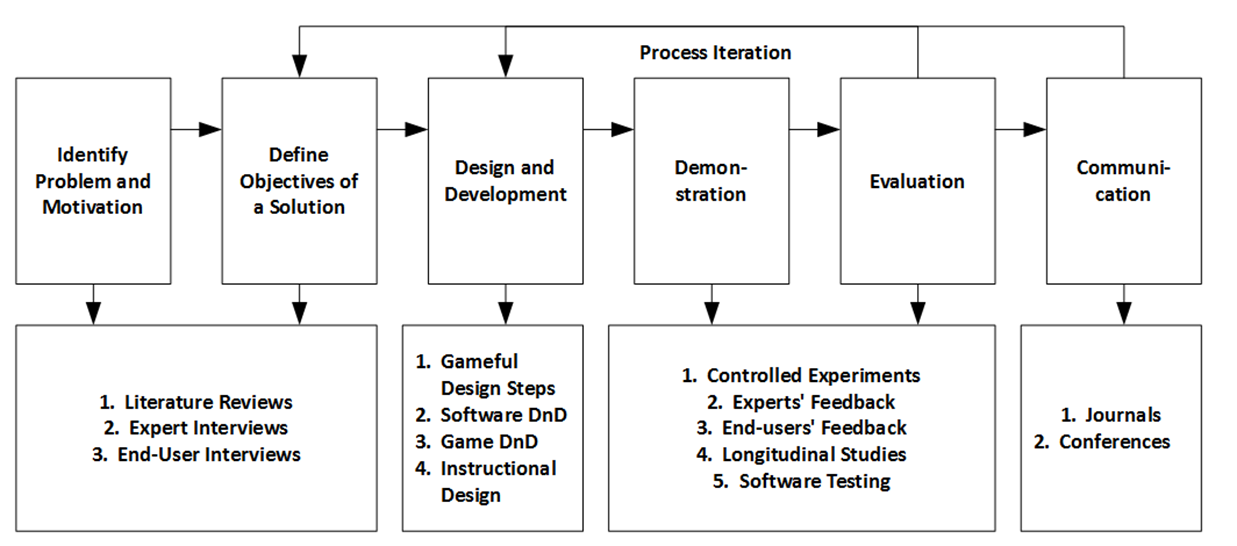
\includegraphics[width=\textwidth]{dsrm}
\caption{Design Science Research Methodology. Adapted from Peffer et al. \cite{peffers2007design}.}
\label{dsrm}
\end{figure}

\section{Research Methods}
\label{Research Methods}
Design Science Research Methodology (DSRM) is selected as the main research method since the main output of this research is a design artefact, a framework to design and generate gamified software modelling learning. DSRM provides a comprehensive conceptual framework and activity guidelines for understanding, developing, executing, and evaluating a design artefact (Figure \ref{dsrm}). Another reason is that it positions itself at the top level of abstraction without going into much detail of how to perform each activity, researches can freely choose other more concrete research methods to carry out the activities. For examples, literature reviews, surveys, or expert interviews can be conducted to determine research problems, motivations, solutions, and objectives as well as controlled experiments to measure and evaluate the effectiveness of the artefacts. DSRM consists of six activities: identify problem and motivation, define objectives for a solution, design and development, demonstration and evaluation, and communication. The progress of this research on these six activities are discussed in the following sections.

\section{Identify Problems and Motivation}
Problem identification and motivation of this research have been largely presented in the Introduction section (Chapter \ref{Introduction}). In this section, they are restated again in a succinct manner. 

Software modelling plays a significant role in software engineering. However, its abstract nature make it challenging to be mastered since most of its concepts are largely presented in symbolical notations. To master software modelling, learners need to posses modelling skills, such as grasping ideas behind models presented in visual modelling notations, presenting back the ideas into visual modelling notations, viewing the ideas from different perspectives using different visual modelling notations, choosing the right levels of abstraction of modelling and moving between. Acquiring these skills might be difficult enough to demotivate learners from learning software modelling.

Apart from the problems previously mentioned, the use of games or game elements rises as solutions to tackle motivational problems. Also, pedagogy has been a mature field to deliver effective learning processes. Therefore, incorporating gameful approaches as well as the pedagogy's best practices can bring great benefits to tackle the problems in learning software modelling. A framework that unify the gameful and pedagogical approaches is needed. This is where Model-Driven Engineering plays it role. Not just being a content in software modelling learning, Model-Driven Engineering provides best practices to automate, customise, and reuse gamified learning activities. Thus, this research is motivated to produce a framework that can support tutors to design gamified learning activities as well as learners to learn software modelling gamefully.


\section{Define Objective for a Solution}
The objective for a solution proposed by this research is to develop a framework that can support tutors to design gamified learning activities as well as learners to learn software modelling in a gamified way. 

To ensure the solution will be fully functioning, some requirements have to be met. So far, these requirements are gathered from two sources, from a preliminary survey (Section \ref{Requirements from Preliminary Survey}) and literature review (Section \ref{Requirements from Literature Review}). These requirements have two roles. First, they provide guidance to design process and, second, they will also act as units of evaluation to confirm the framework meets certain qualities and functionalities. Not all of the requirements have to be satisfied, since they have to be adjusted to the scope of this research. 

A preliminary survey to identify learners' needs, motivations, and challenges has been conducted according to the Research phase of the Deterding's Gameful Design Framework \cite{deterding2015lens}. The preliminary survey aims to identify the requirements in designing the gameful aspect of the framework. It is not intended to measure significance, but it is qualitative investigation to reveal needs, motivations, and challenges in learning software modelling from learners' perspective. The preliminary survey is also in line with the Design Science Research Methodology, in order to identify the problem and motivation so that this research can define objective of a solution accurately in the second activity.

Throughout literature review, requirements was gathered. The requirements are the key points pointed out by Model-Driven Engineering (MDE) experts how MDE should be taught and learned. These requirements are useful in the design of learning contents and activities, the pedagogical aspect, of the framework. From the requirement identification, it is found that the Contents category (Table \ref{table:requirements}) agrees with the item in the Needs category (Table \ref{table:preliminary-survey}). The finding suggests an agreement about the learning contents that should be delivered to students in learning software modelling.

\section{Design and Development}
The design of a design artefact should be rigorously defined. It means the design should be based on existing foundations (models, theories, frameworks, etc.) \cite{von2004design}. Thus, several existing concepts from learning, game, and MDA domains has been applied to design of the framework. There are two parts of the design, the design of gamified learning activities, content structures and order of activities, and the design of the framework so it has capability to deliver the gamified learning activities. The work that have been through to realise such design is explained in the following paragraphs. 

Challenge has been decided as the fundamental game element that exists in the design of the framework since it is one of the key features that exist in every game. Challenge is a crucial game element since it stimulates and provokes a learner to engage with the framework. Challenge can be translated into series of levels with higher levels come with higher difficulties. Thus, the framework should support designers to express such challenge into their gamified learning activity design. One example is to realise learning activities that confirm learning activities in Bloom's taxonomy--remember, understand, apply, analyse, evaluate, and create \cite{krathwohl2002revision}.

While learners are progressing in the framework, they are developing their competence. Thus, difficulty has to be kept balanced with their competence, otherwise they will get bored. It is the situation where the Flow concept \cite{csikszentmihalyi2014toward} can be applied (Figure \ref{learning-models}). To control degree of difficulty, there are three have been identified so far related to pedagogical approach: a combination of Bloom's activities, introduction of new concepts, and application in different domains. The order of the levels of each of the three ways has to be arranged properly following the Flow theory. Concepts that are easier are given earlier than the harder ones, and the difficulty is increased gradually as learners progress. Likewise, Application in the domains that are more familiar with learners should be given first and gradually shifted to the domains that are most unfamiliar (Figure \ref{learning-models}. Combining these three dimensions--types of activities, concepts, and domains--could give us a variety of levels with different degrees of difficulties. The creation of Flow state is not generated automatically by the framework. Instead, tutors are given freedom to define and creatively combine the three dimensions into their learning activity design in order to bring Flow state to learners.

Motivation is an important aspect in the success of learning, and Keller's ARCS motivational model is also selected to address this aspect \cite{keller2010motivational}. The model provides us in each its components---attention, relevance, confidence, satisfaction---a set of predefined techniques to maintain learners' motivation. In a course of a level of framework, there are a start, an end, and learning activities in between (Figure \ref{learning-models}). The ARCS' techniques can be applied to maintain learners' motivation along the course of completing a level. As an example, animation could be used to gain learners' attention, explaining the application of the concept being taught in the currently playing level to give relevance, showing their progress in completing a level to maintain their confidence, and giving them a reward after finishing a level for reward. The incorporation of the ARCS motivational model into the design of the framework is still ongoing.
 
The concept of Scaffolding \cite{vygotsky1978mind, wood1976role} could also be applied to support learners coping challenges (Figure \ref{learning-models}). Throughout finishing a level, scaffolding could be provided in several ways: reducing extensive modelling activities into smaller activity constituents, removing irrelevant activities, providing an almost complete model so they can work on the most relevant activities rather than build the model from scratch, providing help and documentation, and giving some clues of the solutions when they get stuck. This support will be reduced as players progress to maintain the balance between their increasing competence and difficulty. Scaffolding is not generated automatically by the framework. Instead, tutors are given freedom to incorporate scaffolding into their learning activity design. The framework only provide a design environment in which tutors can express scaffolding.

Kolb's experiential learning model \cite{kolb2014experiential} is also applied to the framework. The model agrees knowledge is constructed through experience and based its model on constructivism \cite{kolb2014experiential}. Kolb's model were selected since playing levels in the framework is similar to the learning cycle Kolb proposed. The cycle consists of 4 steps: concrete experience, reflective observation , abstract conceptualisation, and active experimentation. The framework has been designed to allow learners exerting repetitive efforts in order to learn to solve given problems.

The framework has been designed to support tutors to design learning activities that have levels with gradually increasing difficulties as well as variety in challenges, to expose learners to different kinds of domains, models, and diagrams, grasp concepts being taught. Tutorials, another type of game elements \cite{deterding2015lens}, are planned to be embedded into the framework to help learners familiarise themselves with the control system and the flow of the framework. 

The framework has been designed to incorporate interim goal and intrinsic reward game elements \cite{deterding2015lens} to motivate learners. Tutors are supported to model learning patterns for each type of modelling languages (e.g. class diagram, state-chart diagram, and flowchart). A learning pattern will represent a specific case study to introduce learners to particular problems or topics in specific domains or modelling languages. Every pattern will be composed of several activities, which can also be perceived as levels in games, and every activity will have one or more objectives that a learner needs to accomplish to complete it. An activity may also be a continuation of a previous activity, giving the learner step-by-step progression to complete the domain problems. As example, model produced from previous activity will be used as a starting-point model for next activity. Therefore, each learning pattern and activity may introduce new concepts and link them to previously introduced concepts.

A real-world problem can be time-consuming and very complex to model. Thus, the inessential activities that are not significant to the core concepts that are being taught should be excluded \cite{deterding2015lens}. As a result, learners will be more focused on the main concepts. The framework also has been designed to support tutors to embed existing models into their learning activity design so that learners will not have to start modelling from scratch. The following game elements, limited choices (i.e. only limited items can be dragged), microflows (i.e. put the right element to its right place), and bite-sized actions (e.g. drag and drop) \cite{deterding2015lens} are also have been supported to some extends by the framework, depending on how tutors express the design of learning activities, the structure of existing models that are embedded, and the validation of the models. 

Some other game elements that are already part of framework but still need improvement are attractive design and feedback \cite{deterding2015lens}. Attractive design will be improved since it is significant to motivate learners to interact with the framework. The feedback also will be improved so the framework could give instant, noticeable, and actionable feedback to maintain learners' engagement and monitor their progress. Interesting and varied feedback should be designed to appeal to the learners' motives. The details of the application of Deterding's Gameful Design to our design process are presented in Appendix \ref{Application of Deterding's Gameful Design Steps}. The process also produced storyboards that are the preliminary design of levels and graphical user interface of our game (Appendix \ref{Storyboards}). 

The framework has been designed to support modelling in different graphical modelling languages (e.g. UML, BPMN, state-charts), since they are the common languages used in modelling, whether in academia or industry, and extensively used in Model-Driven Engineering. Supporting variety of graphical modelling languages will also minimise bias and ensure the generality of the framework. The framework mimics a graphical modelling tool which learners can perform different kinds of learning activities, from graphically arranging models to meet a set of constraints and requirements to answering multiple choice-like problems.

Model-based approach has been applied so that framework for each graphical modelling language and their learning activities do not have to be developed manually. Instead, tutors only need to model generate them. Using the same approach in Eugenia \cite{kolovos2015eugenia}, metamodel annotations have been used to define the graphical syntaxes of the modelling languages, including an instructional design-like modelling language for tutors to create models of gamified learning activities. Models created using the graphical languages are used to produce models that will be then consumed by a model-to-text transformation to produce gamified learning activities. Thus, the framework supports software modelling tutors in the design and customisation of the framework at the high level of abstraction as well as to automatically build the gamified learning activities. 

The development of prototypes is currently under progress and has been developed using web technologies so that they are accessible to a wide audience. Up to now, it has been able demonstrate one full path from creating a metamodel, creating and validating models that confirms to the metamodel, designing learning activities, reusing the models into the learning activities, generating games based on the learning activity design, and playing the games (see Section \ref{Development} for more detail). 

\section{Demonstration and Evaluation}
This activity has not been executed yet. However, the resulting prototype are planned to be demonstrated and evaluated to computer science students and tutors. Two types of evaluation are planned. First, the evaluation of the learning engagement and performance of the framework. Second, the evaluation of the productivity and maintainability of the framework.

For the engagement and effectiveness evaluation, controlled experiments will be used. The participants, software modelling students, will be divided into two groups, a control group and an experimental group. The control group will learn software modelling using traditional methods, e.g. learning from textbooks, while the experimental group will learn with support from the framework. Then, their learning performance of the two groups will be measured by their ability to solve a set of related modelling problems, while their engagement will be measured using User Engagement Scale \cite{wiebe2014measuring}.  

For the evaluation of the productivity and maintainability of the framework, the participants will be software modelling tutors; they will be divided into two groups, one that will develop framework \emph{with} the framework and one \emph{without} the framework (i.e. using existing web technologies). The execution of the evaluation is similar to the evaluation of Eugenia \cite{kolovos2015eugenia} with appropriate adjustment. They will be asked to design several gamified learning activities in predetermined topics and elaborate the activities into their teaching. After some time, they will be asked to update their  design. The comparison will be on their productivity and the maintainability of their design. To evaluate the generality of the results of both evaluation processes, conducting experiments in different years and countries is also considered.

Additionally, surveying with questionnaires or interviews might be conducted to investigate the underlying variables or processes. Structural equation modelling \cite{hair2016primer} is also an option if measuring the effects of the identified underlying variables is required. An alternative method for understanding of the underlying variables and processes is through investigating the framework's event logs using data mining or machine learning techniques. 

\section{Communication}
The progress of this research should be communicated to a larger audience. So far, only two papers have been made for publication. The first paper has been published in a doctoral symposium setting and the other one is already submitted to conference and waiting for review. The detail of the publication can be found in the Publications section (Chapter \ref{Publications}).

\chapter{Research Plan}
\label{Research Plan}
This year, 2017, time will be spend much on developing prototype with an experiment and a survey in UK will be conducted on between October and December. Next year, 2018, another experiment and survey is also planned to be executed in Indonesia. Year 2019 will be used mostly for thesis writing.

\begin {table}[ht]
\caption {Research Timetable} 
\end{table}
\begin{figure}[ht]
\centering
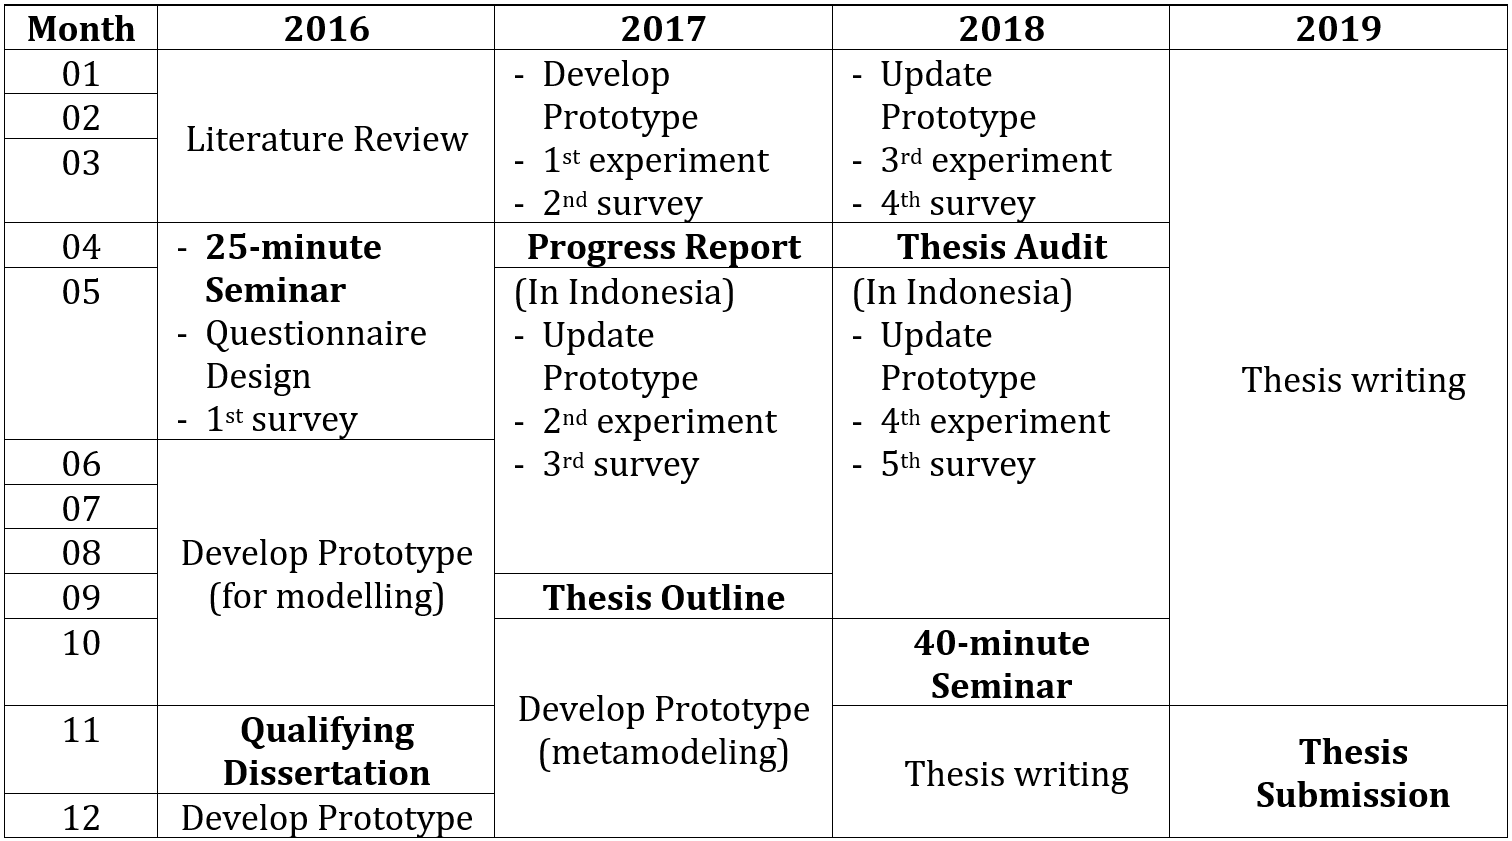
\includegraphics[width=\textwidth]{timetable}
\end{figure}

\chapter{References}
\label{References}

%\addcontentsline{toc}{chapter}{Bibliography}
\begingroup
\bibliographystyle{IEEEtran}
\renewcommand{\chapter}[2]{}%
\bibliography{references}
\endgroup

\chapter{Publications}
\label{Publications}
Papers have been published in the following conferences or journals: 
\begin{enumerate}
 \item A. Yohannis, ``Gamification of software modelling learning,'' in
 \textit{the ACM/IEEE 19th International Conference on Model Driven Engineering Languages and Systems (MODELS 2016) Doctoral Symposium}. CEUR, 2016. \cite{Yohannis2016}.
 \item A. Yohannis, D. Kolovos, and F. Polack, ``Towards Model-Driven Gamified Software Modelling Learning,'' in \textit{the ACM/IEEE 20th International Conference on Model Driven Engineering Languages and Systems (MODELS 2017)}. (submitted, in review).
\end{enumerate}

\begin{appendices}

\chapter{Requirements}
\label{Requirements}

\section{Requirements from Preliminary Survey}
\label{Requirements from Preliminary Survey}
A preliminary survey to identify learners' needs, motivations, and challenges has been conducted according to the Research phase of the Deterding's Gameful Design Framework \cite{deterding2015lens}. The preliminary survey aims to identify the requirements in designing the gameful aspect of the framework. It is not intended to measure significance, but it is qualitative investigation to reveal needs, motivations, and challenges in learning software modelling from learners' perspective. The preliminary survey is also in line with the Design Science Research Methodology, in order to identify the problem and motivation so that this research can define objective of a solution accurately in the second activity. 

Online questionnaires were distributed to students of Model Driven Engineering (MODE) 2015/2016 module. The students were in their Software Engineering master programme at the University of York. From 21 students, only 4 completed the questionnaires. Their responses can be found in Appendix \autoref{chap:Preliminary Survey Data}. Since the number of respondents are small for generalisation, the same survey is planned to applied to next term MODE students.

\textbf{Results}. To identify the learners' needs, respondents were asked two questions. Question 1 aims to identify students' expectations before starting the module, while question 2 aimed at identifying what the students found important after taking the module. Based on the responses, the reasons why the students took MODE module because they wanted to increase their knowledge on Model-Driven Engineering (MDE), possess new advanced skills or abilities and improve their literation of MDE tools. After completing the module, the students valued that the most important lessons were getting new knowledge---domain modelling, metamodel, abstract syntax, abstract thinking, model validation, and the application of models---and skills---generating code, creating DSL, and improving their tool skills. 

Other three questions (Q3-Q5) were also asked the students to identify their motivation in taking MODE module and Learning Model Driven Engineering. Question 3 asked about the reasons behind their decision taking MODE module. Two students stated that they took the module because it is compulsory, but the rest of the students said that they took the module because MDE is an advanced topic and they wanted to see its applicability in the industry and whether it will improve their ability--knowledge and skills.

Question 4 asked the students about what would motivate them more to learn MDE. The students responded that they would be more motivated if they could perceive the advantages of MDE: efficiency and effectiveness it could offer, the benefits of its application in the organisation or real world examples, and its genericity---MDE application in languages other than Java or models other than UML/EMF.

Question 5 asked the students the most basic, underlying motives that make them commit to learning MDE. Substantially, they answered that their main motivation is to gain new ability--knowledge and skills, such as the ability to make an abstraction, advanced skills that are applicable in industry, and knowledge of real-life examples and applications of different models taught in MDE. Nevertheless, passing MODE module, a pragmatical motive, still part of the whole motivation. 

In question 6 and 7, the students were asked about the interesting challenges that they faced during MODE module. They mentioned abstract thinking and model management activities such as defining metamodels, validating model, and how to best model a system---satisfying the model's metamodel and validation so the model could be easily queried and transformed). To overcome challenges, what they did are performing trial-and-error method or experimenting the problems, try many other examples, and completing all the practicals. All of these efforts were summarised as activities to build 'experience'.

Question 8 and 9 were also asked to the students to identify the non-interesting challenges, extraneous challenges that are not relevant to the core activities of modelling. They mentioned following activities: dealing with very specific technical concepts/words that only belong to specific products, focusing too much on how to use tools in other words using very tedious tools or less information on how to use the tools, and judging the quality of a model since there was no explanation of how good of bad the model was. To deal with the uninteresting challenges, they just ignored them, seeking information and solutions from the internet, lecturers, assistants, and discussion groups, and redid building the solutions from the beginning when they had certain problems using the tools.

\textbf{Discussion}. There are few findings from the preliminary interview regarding students' needs, motivations, and challenges, that can be implemented into the design of a framework. \textit{First}, the need of the students to learn MDE is to gain new advanced abilities---knowledge and skills---that are applicable in industry, which, if broken drown, they comprise of model management activities (abstract thinking, modelling, metamodelling, model transformation, validation, and application) and tool literacy. 

\textit{Second}, the motivations of the students to learn MDE are, regardless their view on MODE module as a compulsory module in their programme, they were aware that their motivation should be on satisfying their need in gaining advanced knowledge and skills in MDE as mentioned before, and they would be more motivated if they could perceive the advantages and applicability of MDE, thus showing students the benefits and applications of MDE are crucial in increasing their motivation.

\begin{table}[ht]
\caption{Requirements derived from the preliminary survey.}
\label{table:preliminary-survey}
\begin{center}
\begin{tabular}{ p{2cm}p{1cm}p{10cm} } 
\hline
Category & Code & Requirements from Preliminary Survey \\
\hline
\multirow{1}{2cm}{Needs} 
& RS01 & Teach them knowledge and skills that are applicable in industry: model management (abstract thinking, modelling, metamodelling, model transformation, validation, and application) and tool literacy. \\ 
\hline
\multirow{1}{2cm}{Motivations}
& RS02 & Promote gaining advance knowledge and skills in MDE. \\ 
& RS03 & Promote the benefits and applications of MDE. \\ 
\hline
\multirow{1}{2cm}{Interesting Challenges}
& RS04 & Challenge with model management activities (abstract thinking, model validation, metamodelling, etc.). \\ 
& RS05 & Scaffold learning process to support learners gaining their experience (for an example, dividing the activities into smaller activity chunks). \\ 
\hline
\multirow{1}{2cm}{Un-interesting Challenges}
& RS06 & Increase the usability of the tool being used. \\ 
& RS07 & No need to learn the detailed technical terms specific to certain products. \\ 
& RS08 & Provide documentation and support for the tools being used. \\ 
\hline
\end{tabular}
\end{center}
\end{table}

\textit{Third}, they mentioned model management activities (abstract thinking, model validation, metamodelling, etc.) as the interesting challenges. To overcome the challenges, they did trial-and-error method to gain more experience in overcoming the challenges. These findings are in line with experiential learning which states learning is best achieved through experiencing \cite{kolb2014experiential}. The main concern of gameful design is to reduce the cost of performing such activities so that learners could focus on the core activities without distraction. It could be done by dividing the activities into smaller activity chunks and removing the extraneous, unrelated activities \cite{deterding2015lens}. 

The extraneous, unrelated activities were identified by asking question 8 and 9, which aimed at determining the uninteresting challenges. Most of the complaints were on the tools which were tedious to use. They also argued that there is no need to learn the detailed technical concepts or terms that were only unique to certain products. To overcome the uninteresting challenges, the students preferred to seek information and solutions from on internet, lectures, and discussion groups. Thus, it is paramount to provide comprehensive documentation and support of the tools used in a learning activity \cite{liebel2015ready}. 

\section{Requirements from Literature Review}
\label{Requirements from Literature Review}
Throughout the literature review, requirements was gathered. The requirements are the key points pointed out by Model-Driven Engineering (MDE) experts how MDE should be taught and learned. These requirements are useful in the design of learning contents and activities, the pedagogical aspect, of the framework. Table \ref{table:requirements} is a list of requirements summarised from literature review. 

\begin{table}[ht]\caption{Requirements derived from the literature review.}
\label{table:requirements}
\begin{center}
\begin{tabular}{ p{2cm}p{1cm}p{10cm} } 
\hline
Category & Code & Requirements from Literature Review \\
\hline
\multirow{1}{2cm}{Contents} 
& RL01 & Teach MDE Definition \\ 
& RL02 & Teach semantics, syntaxes, notations \\ 
& RL03 & Teach Modelling, metamodelling, model validation, model transformation\\
& RL04 & Teach the applications of MDE \\
& RL05 & Teach modelling in various domains/contexts \\

\hline
\multirow{1}{2cm}{Priciples and Practices} 
& RL06 & Modelling is abstract thinking \\ 
& RL07 & Object-orientation prerequisite \\
& RL08 & Measure student's model's quality \\
& RL09 & Problem solving first, detail specifications and tools get in the way \\
& RL10 & Provide support to solutions, not answers \\ 
& RL11 & Teach broadly, throughout, not deeply \\
& RL12 & Teach with different modelling languages \\ 
& RL13 & Make it fun \\ 
& RL14 & Teach from ground, real-world objects, up to abstraction \\ 

\hline
\multirow{1}{2cm}{Tool Design}
& RL15 & Support and documentation \\
& RL16 & Build knowledge incrementally \\
& RL17 & Flexibility to explore learning \\
& RL18 & Positive reinforcement \\
& RL19 & Convince of the value of the topic being learned \\ 
& RL20 & High usability \\ 
\hline
\end{tabular}
\end{center}
\end{table}
 
From the requirement identification, it is found that the items in the Contents category (Table \ref{table:requirements}) agrees with the item in the Needs category (Table \ref{table:preliminary-survey}). The finding suggests an agreement about the learning contents that should be delivered to students in learning software modelling.


\chapter{Design and Development}
\label{Design and Development}

The discussion of the design and development of the framework is divided into three sections, the pedagogical aspect design, the game aspect design, and the model-driven aspect design. They are discussed in the following subsections.

\section{Pedagogical Aspect}
Several existing learning concepts are applied in the design process of the framework. In this section, This section explains the relationships between the learning models, their contributions, and how they will be applied to the design of the framework are depicted in in Figure \ref{learning-models} and Figure \ref{learning-models2}.

Challenge is the fundamental game element implemented into the design of our game since it is one of the key features that exist in every game. The challenge is a crucial game element since it stimulates and provokes a player to engage with framework. We translate challenge into series of levels in our design and of course higher levels come with higher difficulty. To realise this, the learning activities---remember, understand, apply, analyse, evaluate, create---from Bloom's taxonomy adopted, since every activity has different cognitive loads according to their order with 'create' has the highest cognitive load. Activity with higher cognitive load is also harder to complete. Therefore, different combinations between the activities can be made so difficulty (cognitive load) increases gradually along the increase of the levels (Figure \ref{learning-models}). Bloom's taxonomy also act as an inventory of activities that provide us many options of activities that could give variability in our design. 

\begin{figure}[ht]
\centering
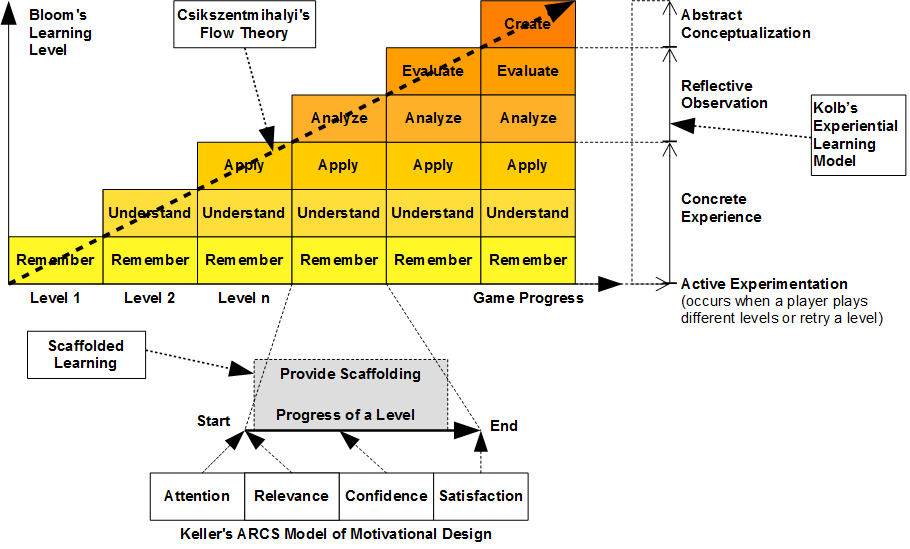
\includegraphics[width=\textwidth]{learning-models}
\caption{Elaborating learning models' contribution to the design of the gamified modeling learning}.
\label{learning-models}
\end{figure}

\begin{figure}[ht]
\centering
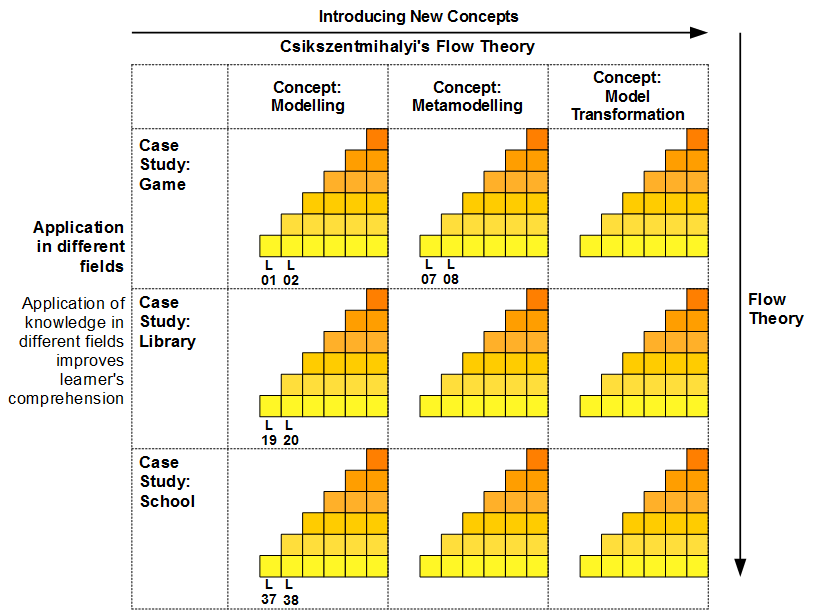
\includegraphics[width=\textwidth]{learning-models2}
\caption{Elaborating learning models' contribution to the design of the gamified modeling learning}.
\label{learning-models2}
\end{figure}

While learners are progressing in the framework, they are developing their competence. Thus, difficulty has to be kept balanced with their competence, otherwise they will get bored. It is the situation where the theory of Flow can be applied (Figure \ref{learning-models}). To control degree of difficulty, there are three ways have been identified so far related to pedagogical approach: a combination of Bloom's activities, the introduction of new concepts, and application in different domains. The order of the levels of each of the three ways has to be arranged properly following the theory of Flow. Concepts that are easier are given earlier than the harder ones, and the difficulty is increased gradually as learners progress. Likewise, Application in the domains that are more familiar with learners should be given first and gradually shifted to the domains that are most unfamiliar (Figure \ref{learning-models}. Combining these three dimensions---types of activities, concepts, and domains---could give us a variety of levels with different degrees of difficulties.

Motivation is an important aspect in the success of learning, Keller's ARCS motivational model are used to address this aspect \cite{keller2010motivational}. The model provides us in each its components---attention, relevance, confidence, satisfaction---a set of predefined techniques to maintain learners' motivation. In a course of a level of framework, there are a start, an end, and learning activities in between (Figure \ref{learning-models}). The ARCS' techniques can be applied to maintain learners' motivation along the course of completing a level. As an example, we could use animation to gain learners' attention, explaining the application of the concept being taught in the currently playing level to give relevance, showing their progress in completing a level to maintain their confidence, and giving them a reward after finishing a level for reward.
 
Scaffolding \cite{vygotsky1978mind, wood1976role} is also applied to support learners coping challenges (Figure \ref{learning-models}). Throughout finishing a level, scaffolding could be provided in several ways: reducing extensive modelling activities into smaller activity constituents, removing irrelevant activities, providing an almost complete model so they can work on the most relevant activities rather than build the model from scratch, providing help and documentation, and giving some clues of the solutions when they get stuck. This support will be reduced as players progress to maintain the balance between their increasing competence and difficulty.

Kolb's experiential learning model is considered to be applied, which is a model that agrees knowledge is constructed through experience and based its model on constructivism \cite{kolb2014experiential}. We select Kolb's model since we perceive that playing a level in framework is similar to the learning cycle Kolb proposed; a cycle consists of 4 steps: concrete experience (CE), reflective observation (RO), abstract conceptualisation (AC), and active experimentation (AE). 

The cycle can be applied to frame learners' activities in gaining new knowledge through solving a problem given in a level. For example, the first time players play a new level, at that moment they encounters a concrete experience (CE). Immediately, they attempt to identify and characterise the problem given in that level and recall any knowledge that is relevant to solve the problem (RO). Next, they construct a solution for the problem that they face (AC). After constructing the solution, they apply the solution to the problem (AE), experience the result (CE), and then evaluate whether the solution solves the problem of the level or not (RO). Any gap that appears will update their knowledge. They use their newly updated knowledge to produce a new solution (AC) that could be applied to the same problem at the same level or different problem in other levels (AE). AE also occurs when players replay the same level or play a similar level they experienced `Game Over' or `Give Up!' decided to choose another level.

\begin{table}[ht]
\caption{Requirements derived from learning theories and models.}
\label{design-learning-models}
\begin{center}
\begin{tabular}{ p{2cm}p{1cm}p{10cm} } 
\hline
Category & Code & Requirements from Learning Models \\
\hline
\multirow{1}{2cm}{Learning Models} 
& RM01 & Design satisfies Bloom's taxonomy. \\
& RM02 & Design suffices Kolb's experiential learning model. \\ 
& RM03 & Design meets Keller's ARCS motivational model. \\
& RM04 & Design fulfils scaffolded learning. \\
& RM05 & Design complies with the theory of Flow. \\ 
\hline
\end{tabular}
\end{center}
\end{table}

Learning activities in Bloom's taxonomy also correspond to the steps in Kolb's learning cycle \cite{murphy2007prior} and both have been applied together to design instructions in different fields \cite{terry1993kolb, howard1996felder, schatzberg2002applying}. Therefore, both could be implemented simultaneously; Bloom's taxonomy provides learning activities while Kolb's model addresses learning cycles in the design of our game. To simplify our work, the elaboration of design and learning models is summarised into a list of requirements (Table \ref{design-learning-models}) that will be used in the design and evaluation activities.

\section{Game Aspect}
In this research, evaluation is planned to assess whether gamification is beneficial for learners of graphical software modelling languages. Graphical modelling languages are selected since they are the common languages used in modelling, whether in academia or industry, and extensively used in Model-Driven Engineering. Standard graphical modelling languages like UML\footnote{\url{http://www.uml.org/}} and BPMN\footnote{\url{http://www.bpmn.org/}}, often used in Model-Driven Engineering, are some of the use-cases. 

Modelling can be expressed in different modelling languages. To minimise bias and ensure the generality of the framework, several graphical modelling languages (e.g. UML, BPMN, state-charts) will be experimented and supported. For each modelling language, the development of dedicated framework that will be derived from the Gameful Design Framework \cite{deterding2015lens} is envisioned. The framework will mimic a graphical modelling tool, and at each level, it will require the learner to graphically construct or adapt a model to meet a set of constraints and requirements.

The framework will have levels of gradually increasing difficulty as well as variety in its challenges, to expose learners to different kinds of domains, models, and diagrams. Tutorials are planned to be embedded into the framework to help learners familiarise themselves with the control system and the flow of the framework. 

The framework will incorporate interim goals and intrinsic rewards to motivate learners. Each type of modelling language (e.g. object modelling, collaboration, process) will have several stories. A story will represent a specific case study to introduce learners to particular problems in specific domains. Every story will be composed of several levels, and every level will have one or more objectives that a learner needs to accomplish to complete it. A level may also be a continuation of a previous level, giving the learner step-by-step progression to complete the domain problems. Each story and level will introduce new concepts and link them with previously introduced concepts.

A real-world problem can be time-consuming and very complex to model. Thus, the inessential activities that are not significant to the core concepts that are being taught should be excluded. As a result, learners will be more focused on the main concepts. Thus, game elements like limited choices (i.e. only limited items can be dragged), microflows (i.e. put the right element to its right place), and bite-sized actions (e.g. drag and drop) will be implemented to facilitate learners in performing the core activities. Likewise, fuzziness will also be used to stimulate learners' creativity since most of the time there is no single correct model for the problem at hand. Attractive design will also be significant to motivate learners to interact with the framework. The framework should be able to give instant, noticeable, and actionable feedback to maintain learners' engagement and monitor their progress. Interesting and varied feedback should be designed to appeal to the learners' motives. This research also plans to implement the framework using web technologies so that they are accessible to a wide audience.

The details of the application of Deterding's Gameful Design to our design process are presented in Appendix \ref{Application of Deterding's Gameful Design Steps}. The process also produced storyboards that are the preliminary design of levels and graphical user interface of our game (Appendix \ref{Storyboards}). 

\section{Model-Driven Aspect}
This research plans to build a framework that will facilitate the design and generation of games for gamified software modeling learning. Rather than developing framework for each graphical modelling language manually, this research will follow a model-based approach. In the spirit of Eugenia \cite{kolovos2015eugenia}, metamodel annotations are used to define the graphical syntaxes of modelling languages and separate models to specify the game elements (constraints, objectives, levels, etc.) of the framework. These models will be then consumed by a model-to-text transformation to produce fully-functional language-specific framework. Thus, the framework supports software modelling tutors in the design and customisation of the framework at the high level of abstraction as well as to automatically build the framework. 

\begin{figure}[ht] \centering 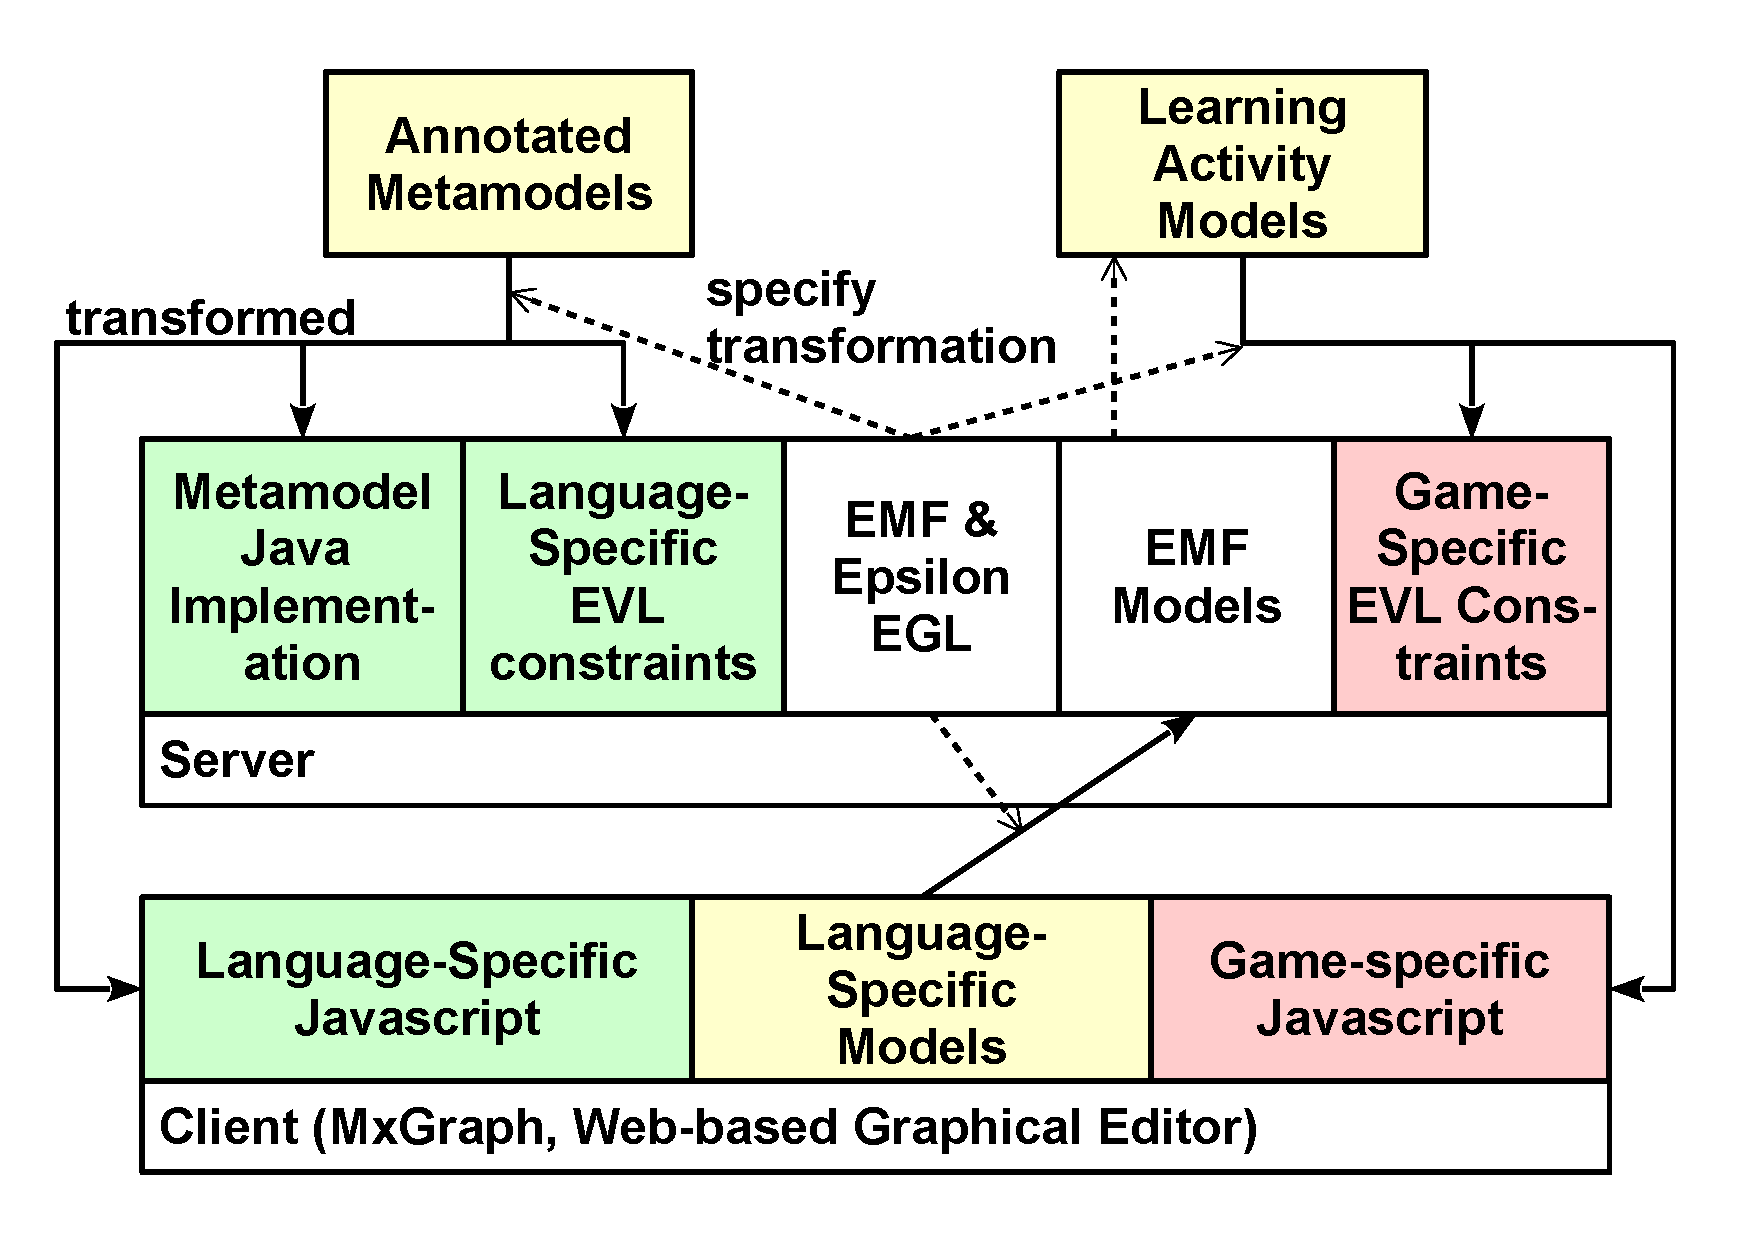
\includegraphics[width=12cm]{artefacts2}
\caption{The main artefacts used in the framework.}
\label{artefact}
\end{figure}

\begin{figure}[ht] \centering 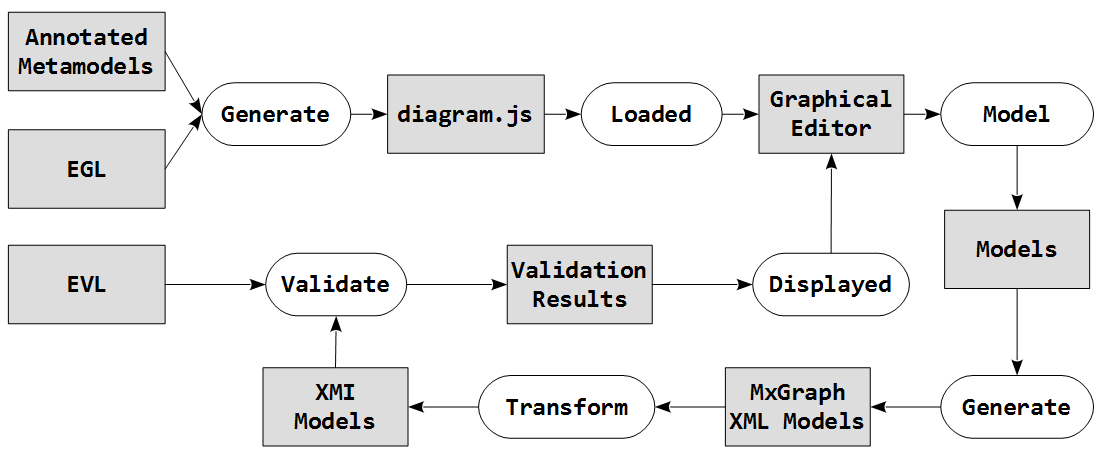
\includegraphics[width=12cm]{work-cycle}
\caption{The process how the framework works from generation of visual modelling notations, modelling on graphical editor, to validation of models.}
\label{work-cycle}
\end{figure}


\chapter{Preliminary Survey Data}
\label{Preliminary Survey Data}

\begin{enumerate}
\item \textbf{If you think back to the time when you were just about to start the MODE module, what did you think you would find interesting in Model ­Driven Engineering?}
\begin{itemize}
\item Learning what MDE actually is. Had never heard of it so was intrigued.
\item I thought I would be provided with a high level approach to designing and managing software/critical systems.
\item Learning some tools to create auto­models.
\item Learning about ways of statically verifying that code conformed to a formal model, and using this to detect and automatically correct bugs learning about ways to automatically modify code based on changes made to a model.
\end{itemize}

\item \textbf{What did you find important in Model­ Driven Engineering?}
\begin{itemize}
\item Domain modelling ­ especially metamodels and the whole concept of abstract syntax. Regarding practicalities, the ability to use models to generate code is the most useful, along with creating DSLs.
\item Trying to learn the specific tools to pass the assessment. Not ideal as I wanted more generic
skill sets in this domain I could apply in my career, instead it was too focused on learning some niche features in Epsilon.
\item abstract thinking ­ validate the models ­ linking the model to real­life.
\item The ability to keep a formal model that the code has been verified to conform to throughout
an entire development process Automatic code generation modifcation based on a model.
\end{itemize}

\item \textbf{ Why did you decide to take the Model ­Driven Engineering module?}
\begin{itemize}
\item It was compulsory. I had no choice.
\item Compulsory.
\item well, I feel that everything around me has a certain model. Therefore, I felt learning about. Model­ Driven will increase my knowledge and experience in work. 
\item It seemed like it would be useful to learn a new approach to software engineering and skills that might be valuable in the industry in the future I was interested in generating and transforming code automatically and using a formal model for the structure of the code.
\end{itemize}


\item \textbf{ What would motivate you more to learn Model Driven Engineering?}
\begin{itemize}
\item Seeing the MDE approach being used to do something that would otherwise be much more tedious to do using more conventional means.
\item To see the benefit applied in the real world and how organisations have benefited from it. Then how can use these skills and adapt them to my needs?
\item If we link it to real­life examples, explore more other tools.
\item More use of it in industry More use with languages other than Java and different types of models such as ones that aren't based on UML/EMF.
\end{itemize}

\item \textbf{ Based on the answers that you’ve provided above (No. 1­4), what were the most basic, core underlying motives or needs that make you commit to learning Model­
Driven Engineering?}

\begin{itemize}
\item The ability to think at a higher level of abstraction and understand the concepts which link together a domain ­ especially, for example, programming languages. 
\item Passing the compulsory paper.
\item see some real­life examples and apply different models to see the differences. 
\item Learning skills which would be valuable in the SE industry in the future Learning something which would help with controlling the complexity of a sofware engineering process by making sure that code
conforms to a formally­defined model
\end{itemize}


\item \textbf{ What were the challenges that you found interesting in learning Model­Driven Engineering? Why?}
\begin{itemize}
\item One of the main challenges is in defining the abstract syntax for a DSL along with placing restrictions on its use through a validation language. There's a balance between trying to make the abstract syntax clean and easy to understand and modify vs. preserving the intended semantics.
\item None really, I found the assignment and practicals a tool based grind as opposed to a useful learning opportunity.
\item I sometimes felt that I could not apply all principles in the practicals­ especially on how we think abstract.
\item Working out how to best model a system, which had been defined informally, in EMF and EVL while keeping all its constraints intact and made it easily queryable and transformable was interesting.
\end{itemize}



\item \textbf{How did you manage to overcome these challenges?}
\begin{itemize}
\item By experimenting and going with what makes the most sense. If it is a structural issue with semantics, it is an abstract syntax issue. If it is something more peculiar, it is a validation issue.
\item By grinding through them.
\item I tried to train myself on other examples, but still, I could not link my models to real­life example( as a real project). 
\item The best way to learn this was from experience which was gained by completing all the practicals.
\end{itemize}


\item \textbf{ What were the challenges---the non­interesting challenges---that hindered or demotivated you in learning Model­Driven Engineering? Why?}
\begin{itemize}
\item Learning the Eclipse Modelling Framework, MOF, etc. wasn't fun. The most fun part was learning and use Emfatic with EGL/EGX and EOL in general. However, actually understanding the meta­metamodel and all the ecore stuff seemed pointless. You do not need to understand what EClass, EEnum, EString etc. are. It is just unnecessary detail that's very specific to
Eclipse and not something that you need to know even if you use Epsilon.
\item The focus on the tool as opposed to the high-level concepts and skill sets that would empower me to utilise Model-Driven Engineering in the real world.
\item sometimes the tool itself, you need to re­track all your changes manually, no right answer or a good explanation why this model is good or bad.
\item Problems using eclipse, the shortcomings of EMF, lack of information available on the internet Eclipse is very large, complex and fragile. EMF/ UML ­style models, can be quite restrictive at times when modelling complex relationships, and often requires resorting to EVL. This is annoying because EVL constraints cannot be easily displayed on a diagram and two different languages/systems, EVL and EMF, are being used for similar things. Sometimes two very similar constraints exist where one can be modelled in EMF, and the other can not, and so requires EVL. Although there is a lot of very good documentation available about the languages in Epsilon, there is far less information on the internet about them than what is usually available for popular programming languages and it would be helpful if there was more.
\end{itemize}

\item \textbf{How did you overcome these challenges?}
\begin{itemize}
\item By ignoring them; once I realised they served no purpose for developers.
\item Reading up about the tools and grinding through them.
\item Asking questions, reading some examples in the Epsilon website forum.
\item Eclipse sometimes stops working but does this usually does not prevent the completion of tasks as most problems can be fixed by deleting the workspace directory and starting again, it simply wastes many time Things that could not be expressed in EMF were instead expressed using EVL. The required information about Epsilon could always be found by
asking classmates and asking lecturers, but this would not be possible if using these languages outside the university
\end{itemize}
\end{enumerate}

\chapter{Application of Deterding's Gameful Design Steps}
\label{Application of Deterding's Gameful Design Steps}


\section{Strategy}
\subsection{Define Target Outcome and Metrics}
\subsubsection{Outcome}
\begin{itemize}
\item Students that use the gamified learning perform better than traditional ones in software modelling.
\end{itemize}

\subsubsection{Metrics}
\begin{itemize}
\item Scores that they get from solving given software modelling problems.
\item Subjective opinions that learning through the gamified systems is better than the traditional ones. 
\item Model metrics of the models that they produce.
\end{itemize}

\subsection{Define Target Users, Context, Activities}
\subsubsection{Users}
Computer Science Undergraduate Students with some knowledge of object-orientation, ideally from both programming and design, and a good understanding of software engineering
\subsubsection{Context}
One term of software modelling course (Time) and in the context of university software modelling course (Place)
\subsubsection{Activities}
Modelling, metamodelling, and model management

\subsection{Identify Constraints and Requirements}
\subsubsection{Laws and regulations}
\begin{itemize}
\item Privacy regulation.
\end{itemize}
\subsubsection{Scope (time, budget, personnel)}
\begin{itemize}
\item Time. One term of software modelling.
\item People. Student of software modelling-related courses.
\item Budget. Available research budget.
\end{itemize}
\subsubsection{Technological requirements}
\begin{itemize}
\item Notebooks, computer desktops.
\item Internet connection.
\end{itemize}
\subsubsection{Others}
\begin{itemize}
\item Align with the existing learning models and software modelling teaching best practices.
\end{itemize}

\section{Research}
\subsection{Translate Users Activities into Behaviour Chains}
\subsubsection{Modelling}
\begin{itemize}
\item Real-world problems are given using textual description (or videos, interviews, images, etc.) 
\item Perform abstraction/identify relevant concepts (objects, values, attributes, and operations) according to the requirements 
\item Translate them into classes and relationships
\item Construct the model in the form of diagrams that represent the classes and relationships in different views (different diagrams)
\item Evaluate the models
\end{itemize}

\subsubsection{Meta-Modelling}
\begin{itemize}
\item Models are given using textual description (or videos, interviews, images, figures, etc.) 
\item Perform abstraction/identify relevant concepts (classes, relationships, attributes) of the models
\item Translate them into metamodel classes
\item Construct metamodel diagrams that represent the metamodel
\item Evaluate the metamodel
\end{itemize}

\subsubsection{Model Management}
\begin{itemize}
\item Problems are given using textual description (or videos, interviews, images, figures, etc.) 
\item Identify goals and constraints
\item Determine the model management operations:
Validation
\item Transformation (model-to-model, text-to-model, model-to-text)
Etc.
\item Refine the operations into more detail steps
\item Test
\item Execute
\end{itemize}

\subsection{Identify User Needs, Motivations, challenges}
\subsubsection{User needs}
\begin{itemize}
\item Master the software modelling.
\end{itemize}
\subsubsection{Motivations}
\begin{itemize}
\item Has competency in software modelling (Ability to solve problems and ability to produce artefacts or concrete products).
\item Fun, challenging.
\item Understanding the importance and advantages of software modelling.
\end{itemize}
\subsubsection{challenges}
\begin{itemize}
\item No fun, the presentation of software modelling is not interesting.
\item Abstraction is difficult, choosing the most relevant elements according to the requirements.
\item Heavy cognitive loads dealing with abstract concepts.
\end{itemize}

\subsection{Determine Gameful Design Fit}
\begin{itemize}
\item Does the activity connect to an actual user need? \textbf{Yes}
\item Is lacking motivation a central issue or opportunity (and not, e.g., poor usability)? \textbf{Both}
\item Does the target activity involve an inherent challenge with a learnable skill? \textbf{Yes}
\item Is affording experiences of competence the most effective and efficient way of improving motivation (and not, e.g., defusing fears)? \textbf{Yes}
\end{itemize}

\section{Synthesis}
\subsection{Formulate Activity, Challenge, Motivation  Triplets for Opportune Activities or Behaviours}

\subsubsection{What motivations energize and direct the activity?}
Software modelling mastery: solving problems and build abstract/concrete artefacts
\subsubsection{What challenges are inherent in the activity?}
\begin{itemize}
\item Abstraction: determine the most relevant objects and relationships between them
\item Diagramming: translate the resulting model into diagram
\item Algorithmic operation: much like programming but for model management
\end{itemize}
\subsubsection{What challenges can be removed through automation or improving usability?} 
\begin{itemize}
\item Simplify the real-world scenario to identify relevant objects
\item Simplify the diagramming processes
\item Simplify the algorithmic operations
\end{itemize}
\subsubsection{What challenges remain that the user can learn to get better at?}
Abstraction, diagramming, algorithmic operation
\subsubsection{What are the activities, challenges, and motives?}
\begin{itemize}
\item Activity: Construct model 
\item Challenge: abstraction, diagramming, algorithmic operation
\item Motive: fear to make mistakes (-), solving problems (+), create artefacts (+)
\end{itemize}

\section{Ideation}
\subsection{Brainstorming Ideas using Innovation Stems}
\subsubsection{Challenge lenses}
Onboarding, scaffolded challenge, varied challenge 
\subsubsection{Goal and motivation lenses}
Interim goals, viral calls to action, next base action, intrinsic rewards, secrets, templates, traces of others
\subsubsection{Action and object lenses}
Bite sized actions, interesting choices, limited choices, micro-flow, small pieces loosely joined, expressive objects, underdetermination, sensual objects
\subsubsection{Feedback lenses}
Immediate, juicy, actionable, appeal to motives, glanceable, varied, surprising, graspable progress.

\subsubsection{Example}
\begin{itemize}
\item Scaffolded challenge lens and Mastery motivation
How might we spark a sense of mastery in abstraction,  diagramming, and model operation?
\item How might we use scaffolded challenge to make the abstraction, diagramming, and model operation more enjoyable?
\item How might we spark a sense of mastery with scaffolded challenge?
\item How might we alleviate fear of making mistakes with scaffolded challenges?
\end{itemize}

\subsection{Prioritise Ideas}
Only one idea created so far. Learners are given a scaffolded series of problems to which they can exercise modelling, metamodelling, and model management. Motivating feedbacks to achieve mastery are integrated as well.

\section{Iterative Prototyping}
Prototyping is still on going work.


\chapter{Storyboard: Object Diagram}
\label{Storyboards}
\begin{itemize}
\item Objects
	\begin{itemize}
	\item Create single object (Level 01)
	\item Create two objects (Level 02)
	\item Create multiple objects (Level 03)
	\end{itemize}
\item Links (Relationships)
	\begin{itemize}
	\item Create single link (Level 04)
	\item Create multiple links (Level 05)
	\end{itemize}
\item Slots (Attributes)
	\begin{itemize}
	\item Determine a slot and its value (Level 06)
	\item Determine slots and their values (Level 07)
	\end{itemize}
\item Operations/Methods
	\begin{itemize}
	\item Determine operation (Level 08)
	\item Determine multiple (Level 09) operations
	\end{itemize}
\item Class of Objects
	\begin{itemize}
	\item Determine the class of homogeneous objects (Level 10)
	\item Determine different classes of heterogeneous objects (Level 11)
	\end{itemize}
\item Case Studies
	\begin{itemize}
	\item Reconstruct the model from the beginning (Level 12)
	\item Apply the skills on different/similar problem (Level 13)
	\end{itemize}
\end{itemize}

\begin{figure}[ht]
    \centering
    \subfloat[Level 01]{{ \frame{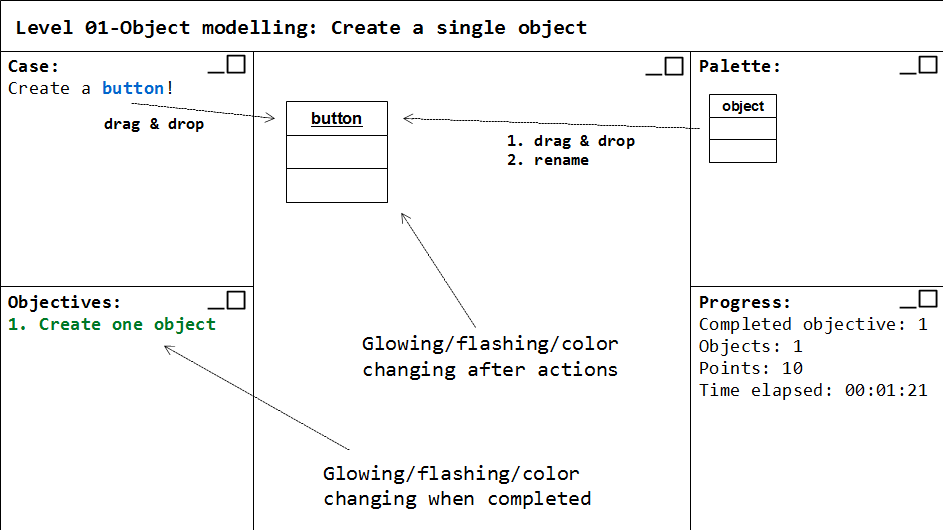
\includegraphics[width=7.16cm]{storyboard01}} }}
    \hspace{0cm}
    \subfloat[Level 02]{{ \frame{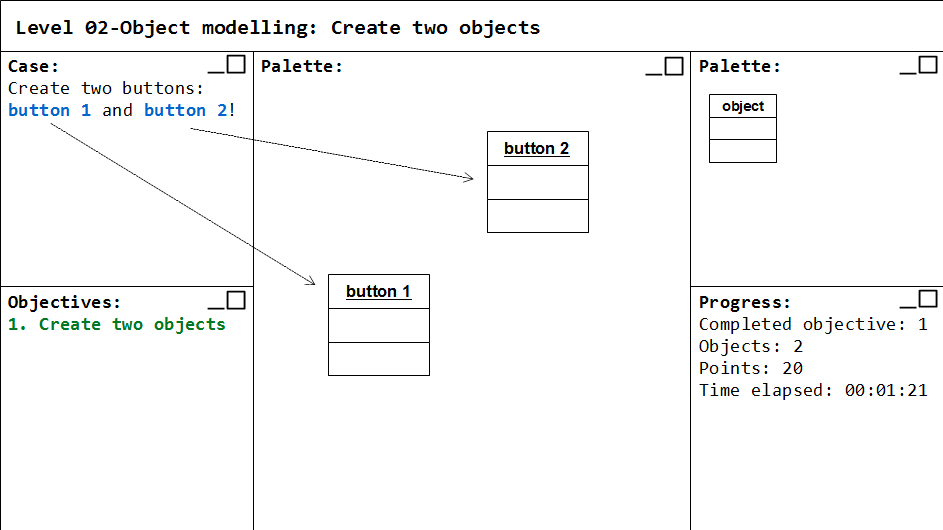
\includegraphics[width=7.16cm]{storyboard02}} }}
    \\
    \subfloat[Level 03]{{ \frame{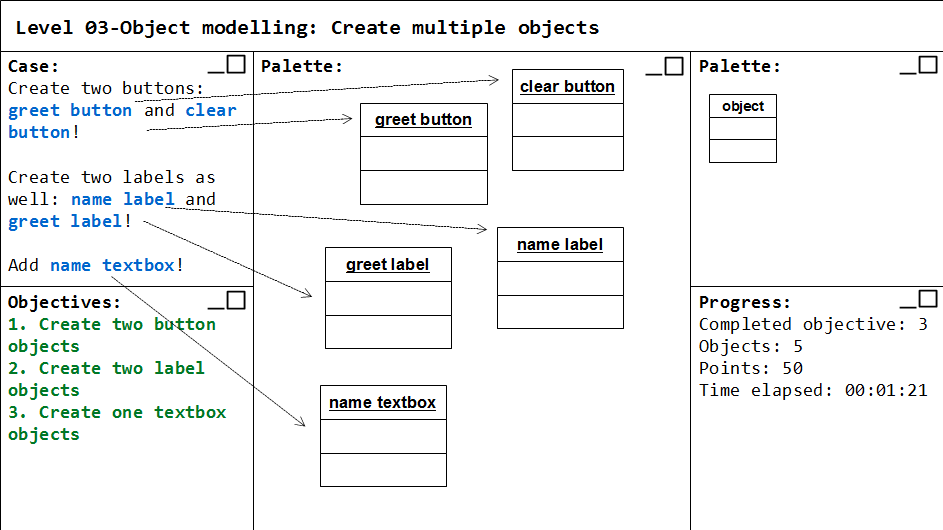
\includegraphics[width=7.16cm]{storyboard03}} }}
    \hspace{0cm}
    \subfloat[Level 04]{{ \frame{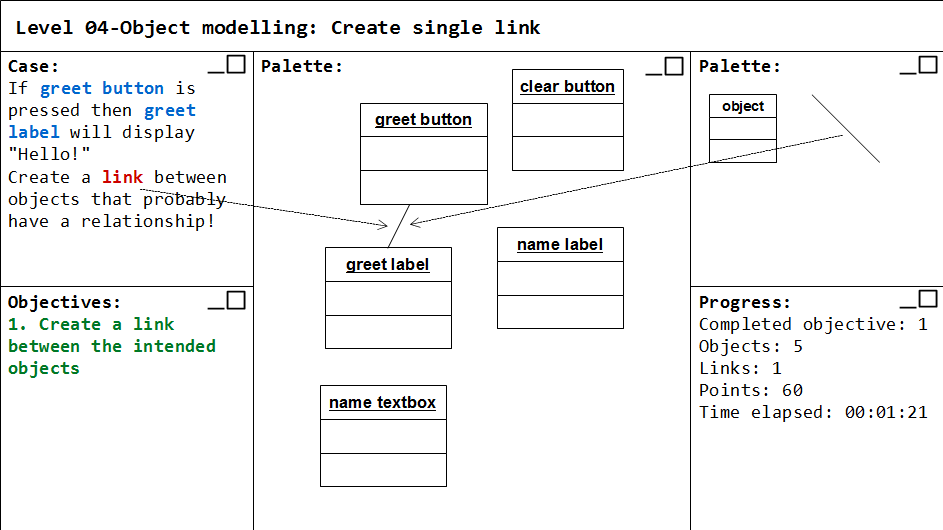
\includegraphics[width=7.16cm]{storyboard04}} }}
    \\
    \subfloat[Level 05]{{ \frame{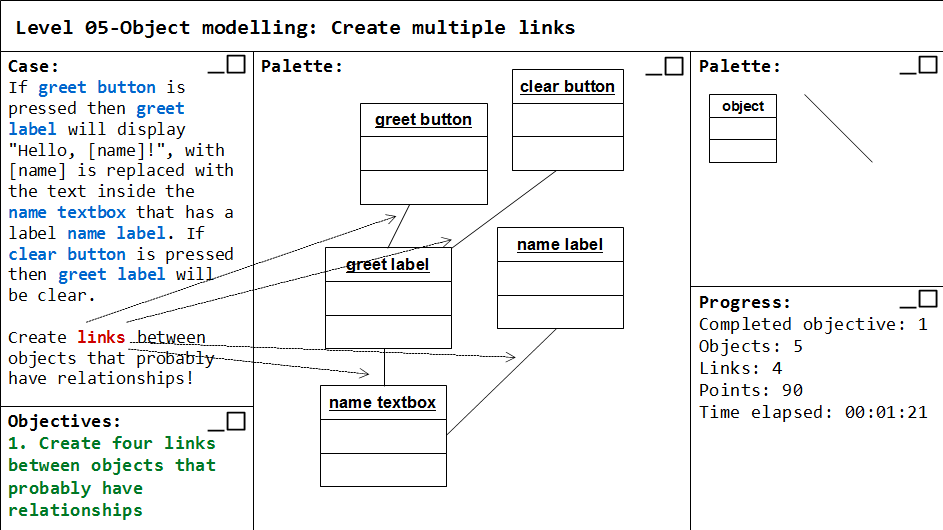
\includegraphics[width=7.16cm]{storyboard05}} }}
    \hspace{0cm}
    \subfloat[Level 06]{{ \frame{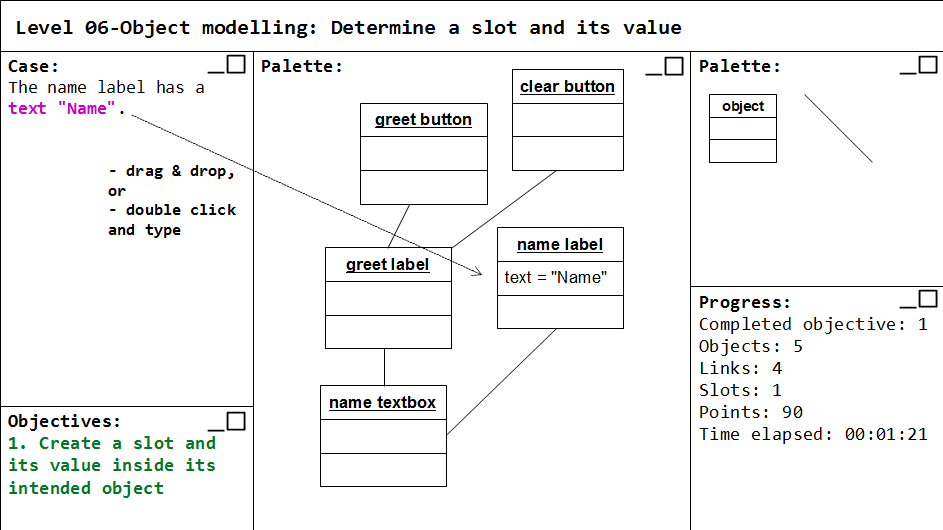
\includegraphics[width=7.16cm]{storyboard06}} }}
    
    
    
    \caption{Storyboard of Gamification of Object Diagram (part 1).}
    \label{storyboard-1}
\end{figure}


\begin{figure}[ht]
    \centering
    \subfloat[Level 07]{{ \frame{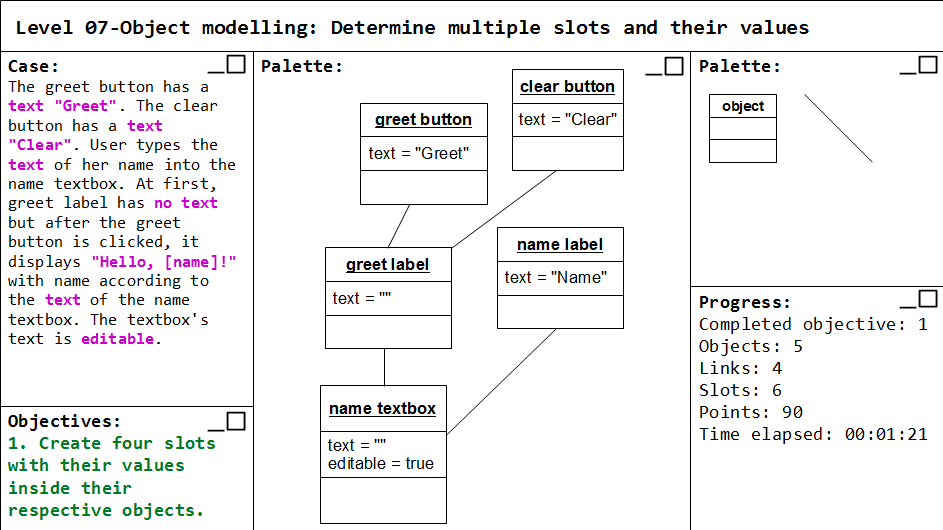
\includegraphics[width=7.16cm]{storyboard07}} }}
    \hspace{0cm}
    \subfloat[Level 08]{{ \frame{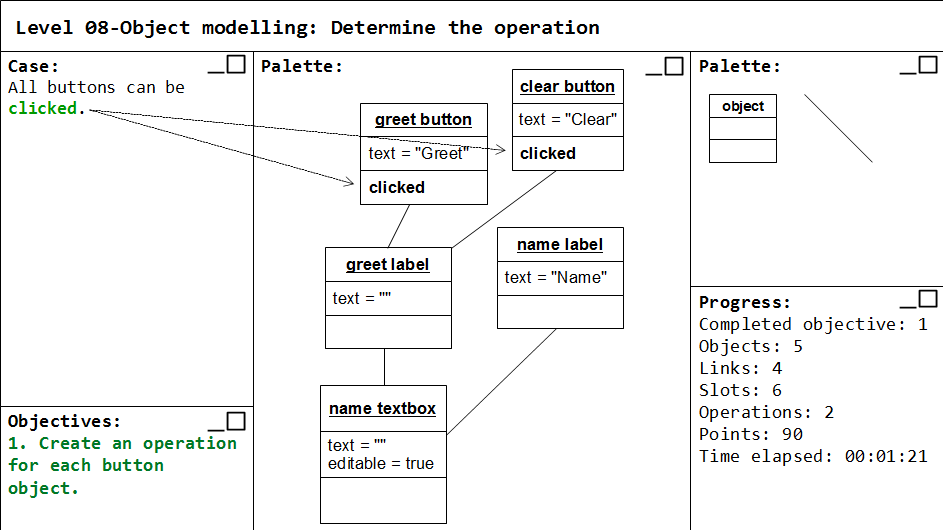
\includegraphics[width=7.16cm]{storyboard08}} }}
    \\
    \subfloat[Level 09]{{ \frame{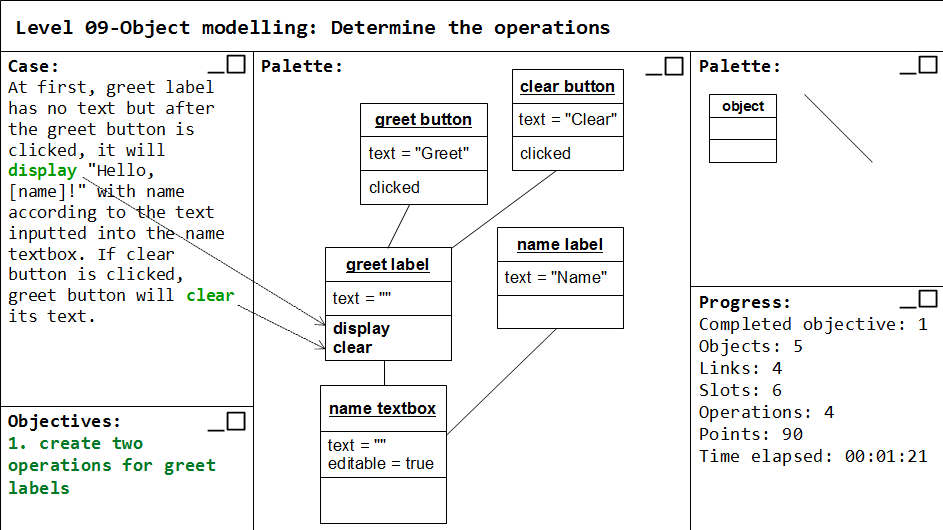
\includegraphics[width=7.16cm]{storyboard09}} }}
    \hspace{0cm}
    \subfloat[Level 10]{{ \frame{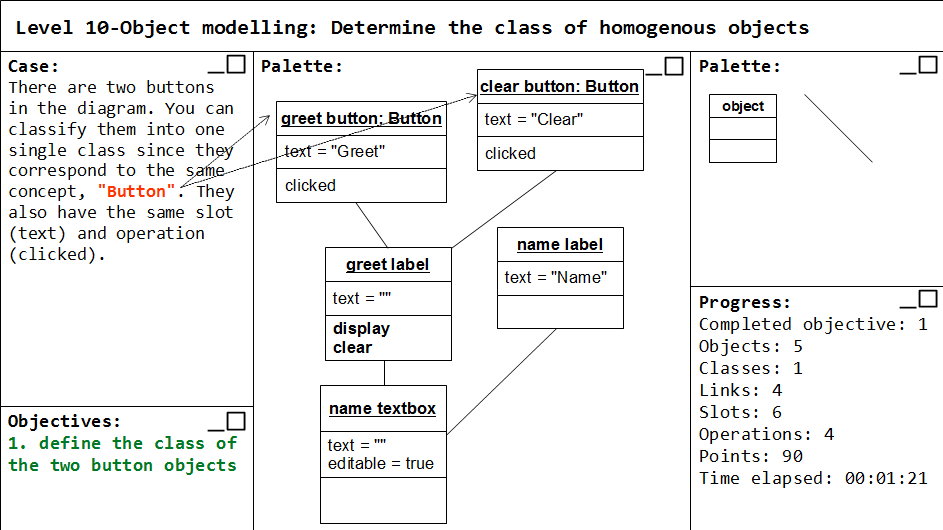
\includegraphics[width=7.16cm]{storyboard10}} }}
    \\
    \subfloat[Level 11]{{ \frame{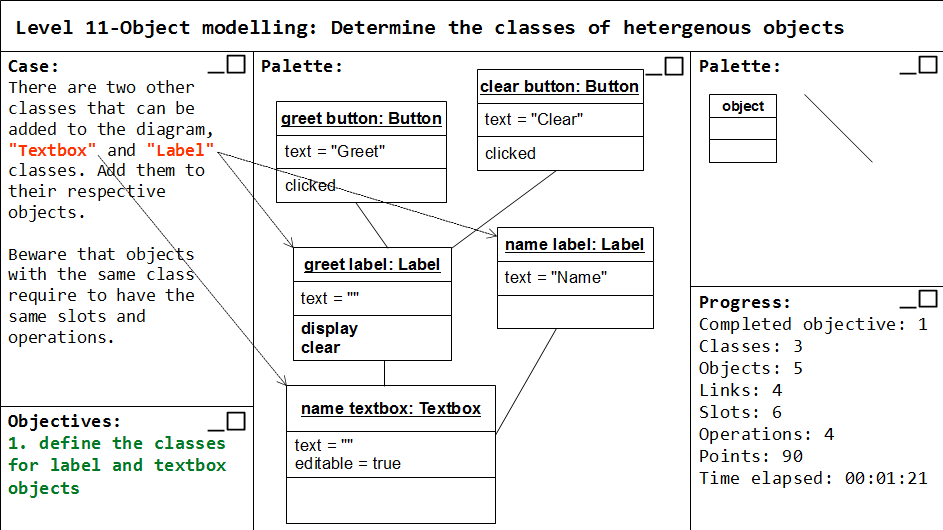
\includegraphics[width=7.16cm]{storyboard11}} }}
    \hspace{0cm}
    \subfloat[Level 12]{{ \frame{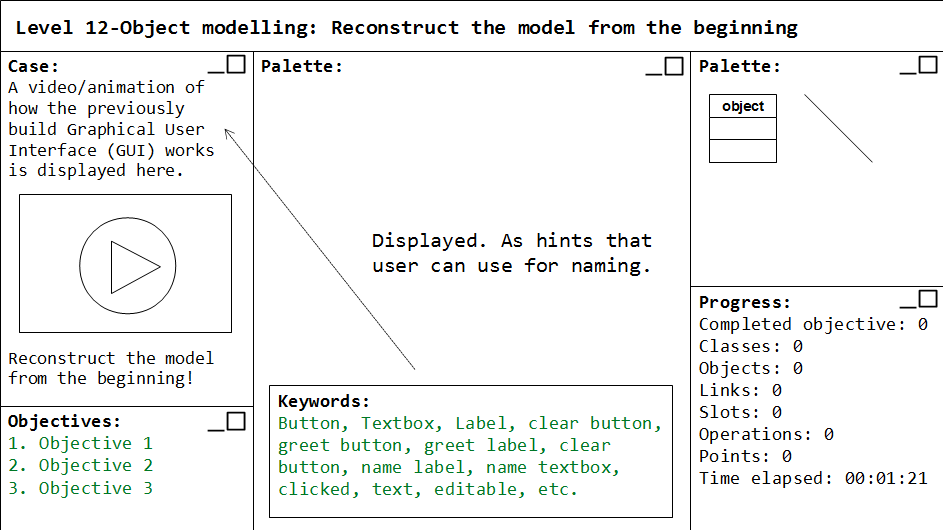
\includegraphics[width=7.16cm]{storyboard12}} }}
\caption{Storyboard of Gamification of Object Diagram (part 2).}
    \label{storyboard-2}
\end{figure}


\end{appendices}

\end{document}





